\documentclass{standalone}
% font set
\usepackage{ctex}
\usepackage{fontspec}
\usepackage[T1]{fontenc}
\usepackage[sc]{mathpazo}
\usepackage{anyfontsize}
\setmainfont{Source Serif 4}
\setsansfont{Source Sans 3}
\setmonofont{Menlo}
\setCJKmainfont[BoldFont=黑体-简 中等,ItalicFont=楷体-简 常规体]{宋体-简 常规体}

% colors
\usepackage[dvipsnames]{xcolor}
\definecolor{pku-red}{RGB}{139,0,18}
\usepackage{colortbl}
\newcommand{\light}[1]{\textcolor{Orchid}{#1}}
\newcommand{\contrastlight}[1]{\textcolor{TealBlue}{#1}}

% plots
\usepackage{tikz}
\usepackage{tikz-cd}
\usetikzlibrary{arrows}
\usetikzlibrary{arrows.meta,positioning,calc,3d,backgrounds,fit}
\usetikzlibrary{automata}
\usepackage{pgfplots}
\pgfplotsset{compat=newest}
\tikzset{
    punkt/.style={
        rectangle,
        rounded corners,
        draw=black, very thick,
        minimum height=2em,
        inner sep=6pt,
        text centered,
        fill=gray!30
    }
}

% math package
\let\Bbbk\relax
\usepackage{amsmath}
\usepackage{mathrsfs}
\usepackage{amssymb}
\usepackage{amsfonts}
\usepackage{stmaryrd}
\usepackage{latexsym}
\usepackage{extarrows}
\SetSymbolFont{stmry}{bold}{U}{stmry}{m}{n}


\begin{document}
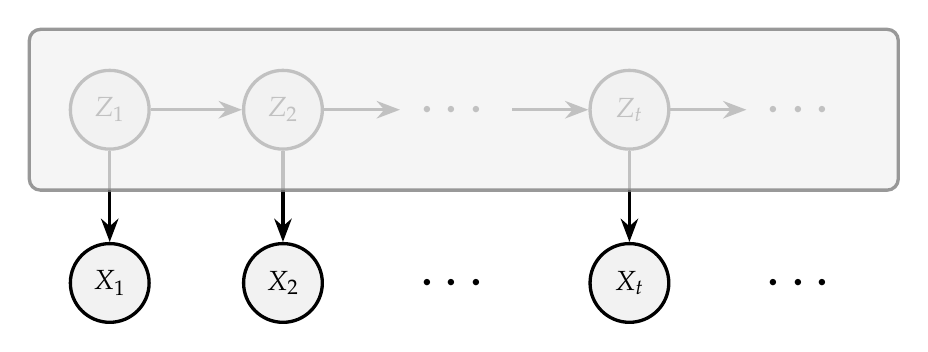
\begin{tikzpicture}[node distance=2.2cm, every state/.style={minimum size=1cm, very thick, fill=gray!10}, auto]

    % States
    \node[state] (Z1) {$Z_1$};
    \node[state] (Z2) [right of=Z1] {$Z_2$};
    \node (dots) [right of=Z2, scale=2] {$\dots$};  % Increased size of dots
    \node[state] (Zt) [right of=dots] {$Z_t$};
    \node (dots1) [right of=Zt, scale=2] {$\dots$};  % Increased size of dots
    \node[state] (X1) [below of=Z1] {$X_1$};
    \node[state] (X2) [right of=X1] {$X_2$};
    \node (dots2) [right of=X2, scale=2] {$\dots$};  % Increased size of dots
    \node[state] (Xt) [right of=dots2] {$X_t$};
    \node (dots3) [right of=Xt, scale=2] {$\dots$};  % Increased size of dots

    % Transitions outside the box
    \path[->, >={Stealth},very thick] 
    % From state 0 to state 1
    (Z1) edge node {} (Z2)
    (Z2) edge node {} (dots)
    (dots) edge node {} (Zt)
    (Zt) edge node {} (dots1)
    (Z1) edge node {} (X1)
    (Z2) edge node {} (X2)
    (Zt) edge node {} (Xt);

    % Hidden state box with gray and opacity
    \begin{scope}[gray, opacity=0.8] % Set gray and opacity
        \node[draw=gray, very thick, fill=gray!10, rounded corners, fit=(Z1) (Z2) (Zt) (dots1), inner sep=0.5cm] {};
    \end{scope}



\end{tikzpicture}


\end{document}